\documentclass[aspectratio=169]{beamer}
\usepackage{framed}
\usepackage{lhps}
\usepackage{pifont}

\renewcommand{\ImageSource}{L2-Images/}
\begin{document}

\section{Что такое деконструкция?}

\begin{Person}{Derrida}{Жак Деррида}{1930--2004}
Деконструкция \only<2-3>{---} \only<2>{...}\uncover<3>{не метод, не критика, не анализ}
\end{Person}

\begin{frame}
Деконструкция -- направление постмодернистского критицизма, связываемое с работами Деррида. Являясь попыткой радикализации хайдеггеровской деструкции западноевропейской метафизики, Деконструкция имеет целью не прояснение фундаментального опыта бытия, но всеобъемлющую негацию понятия бытия как такового. Деконструкция постулирует принципиальную невозможность содержательной экспликации бытия: тематика субъективирующей интериоризации не случайно является для нее главной. Критика основополагающих концептов традиционной философии (в границах которой — несмотря на непосредственное влияние на становление деконструктивизма -- для Деррида остаются и Ницше, и Фрейд, и Гуссерль, и Хайдеггер) -- <<присутствия>>, <<действительности>>, <<тождества>>, <<истины>> -- исходит из посылки, что статус рационального в культуре не самовоспроизводится на собственном материале, но поддерживается постоянным усилием по вытеснению из его сферы элементов, оказывающихся не-мыслью, не-мыслимым. Эта репрессивная интенция, лежащая в основании западноевропейской культуры, обозначается Деррида как логоцентризм. Именно системное опровержение философии/культуры логоцентризма суть пафосная  программа Деконструкции.
\end{frame}

\begin{Person}{deMan}{Поль де Ман}{1919 -- 1983}
\Citation{
Из опыта чтения абстрактных философских текстов нам всем знакомо облегчение, которое мы чувствуем, когда рассуждение сменяется тем, что называется <<конкретным примером>>. Однако именно в этот самый момент, когда нам наконец кажется, что мы все поняли --- мы, в действительности, дальше от понимания, чем когда-либо прежде}{}
\end{Person}

\begin{frame}
\begin{center}
\begin{tikzpicture}[x=3cm,y=-0.9cm]
\uncover<+->{\node at (-1,-1) {
\includegraphics[angle=10, width=7cm]{L2-Images/nose1.jpg}};}
\uncover<+->{\node at (1,-1) {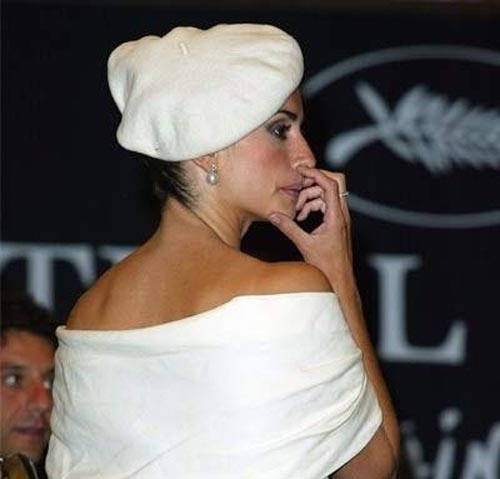
\includegraphics[angle=-5, width=7cm]{L2-Images/nose3.jpg}};}
\uncover<+->{\node at (1,1) {
\includegraphics[angle=3, width=7cm]{L2-Images/nose2.jpg}};}
\uncover<+->{\node at (-1,1) {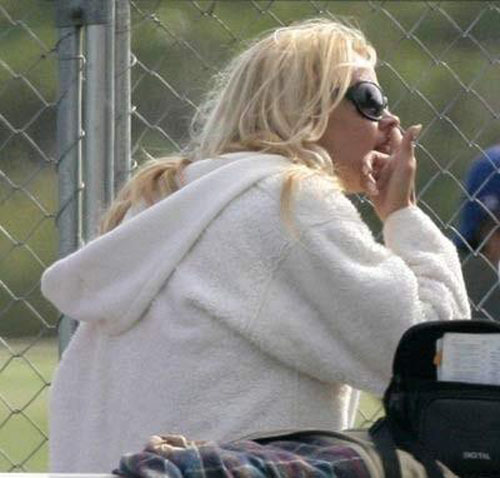
\includegraphics[angle=-2, width=7cm]{L2-Images/nose4.jpg}};}
\uncover<+->{\node at (0,0) {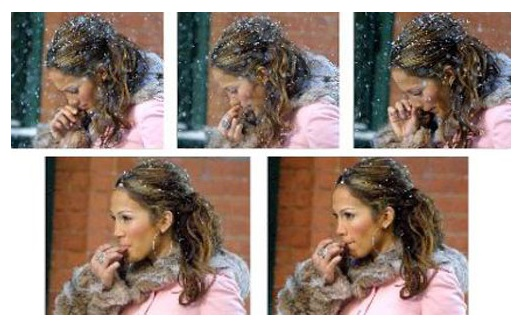
\includegraphics[width=10cm]{L2-Images/nose5.jpg}};}
\end{tikzpicture}
\end{center}
\end{frame}


\begin{frame}
\begin{center}
\begin{huge}
Нельзя публично ковырять в носу!
\end{huge}
\end{center}
\end{frame}

\begin{Person}{freud}{Зигмунд Фрейд}{1856 -- 1939}
\footnotesize{
\begin{tabular}{c c c c}
& \uncover<15->{Ребенок} & \uncover<15->{Взрослый} & \uncover<15->{Родитель} \\
& \uncover<3->{Оно} & \uncover<7->{Я} & \uncover<11->{Сверх-Я} \\
& \uncover<4->{Ид} & \uncover<8->{Эго} & \uncover<12->{Супер-Эго} \\
\uncover<2->{Подсознательное} & \uncover<5->{\normalsize\checkmark} &\uncover<9->{\normalsize\ding{55}} & \uncover<13->{\normalsize\checkmark}\\
\uncover<2->{Сознательное} & \uncover<6->{\normalsize\ding{55}} & \uncover<10->{\normalsize\checkmark} &  \uncover<14->{\normalsize\checkmark}
\end{tabular}}
\end{Person}

\usetikzlibrary{calc}


\begin{frame}
\begin{tikzpicture}[x=3cm,y=-3cm]
\draw (0,0) circle (1);
\uncover<2->{\draw (-1,0) -- node[above] {Нельзя публично ковырять в носу} (1,0);}
\uncover<3->{\node at (0,0.5) {Оно};}
\uncover<4->{\node at (0,-0.5) {Я};} 
\uncover<5->{\draw (-1,0) -- node[below] {Сверх-Я} (1,0);}

\uncover<6>{
\draw[dashed] (-2.5,-0.25) -- node[below] {Бессознательное} (-1,-0.25) -- (1,-0.25);
\draw[dashed] (-2.5,-0.25) -- node[above] {Сознательное} (-1,-0.25) -- (1,-0.25);
}

\uncover<7>{
\draw[dashed] (-2.5,0.25) -- node[below] {Бессознательное} (-1,0.25) -- (1,0.25);
\draw[dashed] (-2.5,0.25) -- node[above] {Сознательное} (-1,0.25) -- (1,0.25);
}
\end{tikzpicture}
\end{frame}

\begin{frame}
\begin{center}
\begin{tikzpicture}[x=1.5cm,y=1.5cm]
\node(n0) at (-2,0) {Можно};
\node(n1) at (2,0) {Нельзя};
\node(n2) at (0,2) {Публично};
\node(n3) at (0,-2) {Непублично};
\draw(n0) -- (n1);
\draw(n2) -- (n3);
\uncover<2->{\node at(1,1) {Автор};}
\uncover<3->{\node[align=center] at(-1,1) {Вытесненная\\ субличность};}
\uncover<4-5>{\node at(1,-1) {Автор};}
\uncover<5>{\node[align=center] at(-1,-1) {Вытесненная\\ субличность};}
\uncover<6->{\node[align=center] at(-1,-1) {Неактуальная\\ субличность};}
\uncover<7>{\node[align=center] at(1,-1) {Бессмыслица};}
\uncover<8>{\node[align=center] at(1,-1) {Вытесненная\\ субличность};}
\end{tikzpicture}
\end{center}
\end{frame}

\begin{frame}
\begin{center}
\begin{small}
\begin{tikzpicture}[x=3cm,y=-1.5cm]
\node (n0) at (0,0) {Нельзя публично ковырять в носу};

\uncover<2->{
\node (n1) at (-1,1) {можно/нельзя};
\node[align=center] (n2) at (0,2) {публично/\\непублично};
\node[align=center] (n3) at (1,1) {ковырять в носу/\\не ковырять в носу};
\draw (n0) -- (n1);
\draw (n0) -- (n2);
\draw (n0) -- (n3);
}
\uncover<3->{
\node[align=center] (n31) at (1,2) {нарушать/не нарушать\\ телесные границы};
\node (n32) at (2,2) {нос/не нос};
\draw (n3) -- (n31);
\draw (n3) -- (n32);
}
\uncover<4->{
\node[align=center] (n11) at (-2,2) {доминирование/\\унижение};
\node[align=center] (n12) at (-1,2) {разрешение/\\запрещение};
\draw (n1) -- (n11);
\draw (n1) -- (n12);
}
\uncover<5->{
\node (n21) at (-2,3) {охранник};
}
\uncover<6->{
\node (n22) at (-1,3) {запрещальщик};
}
\uncover<7->{
\node (n23) at (0,3) {актер};
}
\uncover<8->{
\node (n24) at (1,3) {футляр};
}
\uncover<9->{
\node (n25) at (2,3) {цензор};
}
\uncover<10>{
\node (x) at (0,4) {Можно публично ковырять в носу};
}

\uncover<11>{
\node (x3) at (0,4) {Нельзя ковырять в носу {\bf наедине с собой}};
\draw (n23) -- (x3);
}

\uncover<12>{
\node (x4) at (0,4) { Нельзя публично {\bf не нарушать телесные границы} };
\draw (n24) -- (x4);
}

\uncover<13>{
\node (x5) at (0,4) { Нельзя публично ковырять {\bf не в носу}  };
\draw (n25) -- (x5);
}

\uncover<14>{
\node (x2) at (0,4) { {\bf Я обязан} публично ковырять в носу  };
\draw (n22) -- (x2);
}
\uncover<15>{
\node (x1) at (0,4) { {\bf Ты не запрещаешь} мне публично ковырять в носу  };
\draw (n21) -- (x1);
}
\end{tikzpicture}
\end{small}
\end{center}
\end{frame}


\begin{frame}
\only<1>{Вечером, окончив работу, она забиралась в уголок возле камина и сидела там на ящике с золой. Поэтому сестры, а за ними и все в доме прозвали ее Золушкой.}

\uncover<2->{Вечером, окончив работу, он забирался в уголок возле камина и сидел там на ящике с золой. Поэтому братья, а за ними и все в доме прозвали его Золушком.\\[0.5cm]}

\uncover<3->{А все-таки Золушек в своем стареньком костюмчике, перепачканном золою, {\bf был во сто раз милее}, чем его братцы, разодетые в бархат и шелк.\\[0.5cm]}

\uncover<4->{И вот как-то раз сын короля той страны устроил большой бал и созвал на него {\bf всех знатных людей с мужьями и сыновьями.}\\[0.5cm]}

\uncover<5->{Отчим и братья уехали. Золушек долго смотрел им вслед, а когда их карета исчезла за поворотом, {\bf он закрыл лицо руками и горько заплакал.}}

\end{frame}

\begin{bframe}
\begin{itemize}
\item Красота
\item Общественная значимость
\item Выражение эмоций
\end{itemize}
\end{bframe}

\begin{frame}
\uncover<1->{... Но придворный кавалер, который примерял туфельку, внимательно посмотрел на Золушку и, заметив, что она {\bf весьма безобразна}, сказал:\\[0.2cm]}

\only<2>{
-- Я получил приказание от принца примерить туфельку всем девушкам в городе. Позвольте вашу ножку, сударыня!}

\uncover<3->{
-- Я получил приказание от принца примерить туфельку всем девушкам в городе. Позвольте вашу {\bf ножищу}, сударыня!\\[0.2cm]
}
\uncover<4->{
Он усадил Золушку в кресло и, надев хрустальную туфелищу на ее гигантскую ножищу, сразу увидел, что больше примерять ему не придется: башмачище был точь-в-точь по ножище, а ножище -- по башмачищу.\\[0.2cm]}
\only<5>{
В эту самую минуту дверь отворилась, и в комнату вошла фея -- Золушкина крестная.}
\uncover<6->{
В эту самую минуту дверь отворилась, и в комнату {\bf прошаркала ведьма} -- Золушкина крестная.\\[0.2cm]}

\uncover<7->{
Она дотронулась своей волшебной палочкой до нарядного платья Золушки, и оно стало еще более {\bf убогим и безобразным}, чем было накануне на балу.\\[0.2cm]}

\uncover<8->{
Ее отвезли во дворец к молодому принцу, который нашел, что она стала {\bf еще отвратительнее}, чем была прежде.\\[0.2cm]
}

\uncover<9->{
\bf А через несколько дней сыграли веселую свадьбу.
}
\end{frame}



\end{document}